\documentclass[tikz,border=12pt]{standalone}
\usepackage[T1]{fontenc}
\usepackage{mathpazo}
\usepackage{amsmath,amssymb}
\usetikzlibrary{arrows.meta, positioning, calc, fit, decorations.pathreplacing}

\definecolor{stblue}{HTML}{7B97AD}
\definecolor{rwgold}{HTML}{B8995E}
\definecolor{sage}{HTML}{7A9A7E}
\definecolor{dkbrown}{HTML}{3D3530}
\definecolor{wmgray}{HTML}{7B7067}
\definecolor{cream}{HTML}{F9F6F0}
\definecolor{border}{HTML}{D4C9B8}
\definecolor{terracotta}{HTML}{C47A6A}
\definecolor{lavender}{HTML}{907EA0}

\begin{document}
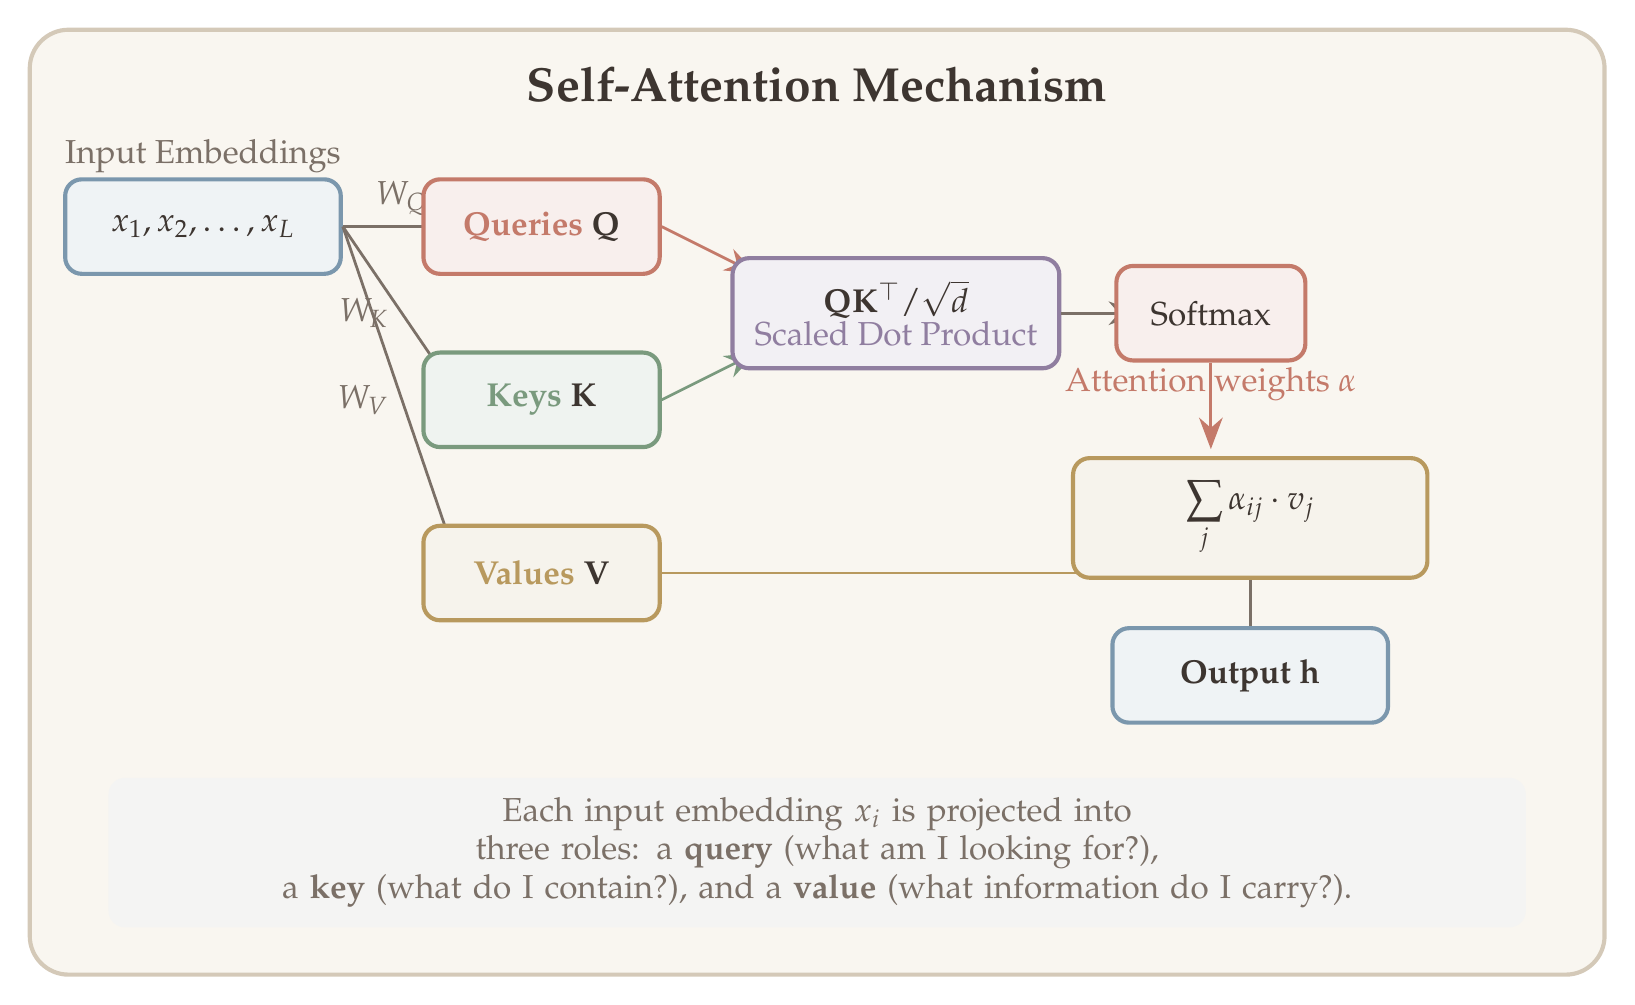
\begin{tikzpicture}[
  >={Stealth[length=4mm, width=3mm]},
  every node/.style={text=dkbrown, font=\large},
  box/.style={rounded corners=6pt, line width=1.5pt, minimum height=1.2cm, align=center, inner sep=8pt},
]

% Background
\fill[cream, rounded corners=14pt] (0,0) rectangle (20,12.0);
\draw[border, line width=1.5pt, rounded corners=14pt] (0,0) rectangle (20,12.0);

% Title
\node[font=\LARGE\bfseries, text=dkbrown] at (10,11.3) {Self-Attention Mechanism};

% Input embeddings box
\node[box, fill=stblue!12, draw=stblue, minimum width=3.5cm] (input) at (2.2,9.5) {$x_1, x_2, \ldots, x_L$};
\node[font=\large, text=wmgray] at (2.2,10.4) {Input Embeddings};

% Three projection arrows
\draw[wmgray, line width=1pt, ->] (input.east) -- ++(1.5,0) node[midway, above, font=\large, text=wmgray] {$W_Q$} coordinate (qstart);
\draw[wmgray, line width=1pt, ->] (input.east) -- ++(1.5,-2.2) node[midway, left, font=\large, text=wmgray, xshift=-1pt] {$W_K$} coordinate (kstart);
\draw[wmgray, line width=1pt, ->] (input.east) -- ++(1.5,-4.4) node[midway, left, font=\large, text=wmgray, xshift=-1pt] {$W_V$} coordinate (vstart);

% Q box
\node[box, fill=terracotta!12, draw=terracotta, minimum width=3.0cm] (Q) at (6.5,9.5) {{\bfseries\color{terracotta}Queries} $\mathbf{Q}$};

% K box
\node[box, fill=sage!12, draw=sage, minimum width=3.0cm] (K) at (6.5,7.3) {{\bfseries\color{sage}Keys} $\mathbf{K}$};

% V box
\node[box, fill=rwgold!12, draw=rwgold, minimum width=3.0cm] (V) at (6.5,5.1) {{\bfseries\color{rwgold}Values} $\mathbf{V}$};

% Q and K merge into dot product
\draw[terracotta, line width=1pt, ->] (Q.east) -- ++(1.2,-0.6) coordinate (dp1);
\draw[sage, line width=1pt, ->] (K.east) -- ++(1.2,0.6) coordinate (dp2);

% Scaled dot product box
\node[box, fill=lavender!12, draw=lavender, minimum width=3.8cm] (sdp) at (11.0,8.4) {%
  $\mathbf{Q}\mathbf{K}^\top / \sqrt{d}$\\[-2pt]
  {\color{lavender}Scaled Dot Product}
};

% Arrow to softmax
\draw[wmgray, line width=1pt, ->] (sdp.east) -- ++(1.0,0);

% Softmax box
\node[box, fill=terracotta!12, draw=terracotta, minimum width=2.4cm] (sm) at (15.0,8.4) {Softmax};
\node[font=\large, text=terracotta] at (15.0,7.5) {Attention weights $\alpha$};

% Arrow from softmax down
\draw[terracotta, line width=1pt, ->] (sm.south) -- ++(0,-1.1);

% V arrow to weighted sum
\draw[rwgold, line width=1pt, ->] (V.east) -- (13.5,5.1) -- (13.5,5.7);

% Weighted sum box
\node[box, fill=rwgold!12, draw=rwgold, minimum width=4.5cm] (ws) at (15.5,5.8) {$\displaystyle\sum_j \alpha_{ij} \cdot v_j$};

% Output arrow
\draw[wmgray, line width=1pt, ->] (ws.south) -- ++(0,-1.0);

% Output box
\node[box, fill=stblue!12, draw=stblue, minimum width=3.5cm] (output) at (15.5,3.8) {{\bfseries Output} $\mathbf{h}$};

% Annotation box at bottom
\fill[wmgray!8, rounded corners=6pt] (1.0,0.6) rectangle (19.0,2.5);
\node[text width=16cm, align=center, font=\large, text=wmgray] at (10,1.55) {%
  Each input embedding $x_i$ is projected into three roles: a \textbf{query} (what am I looking for?),\\
  a \textbf{key} (what do I contain?), and a \textbf{value} (what information do I carry?).};

\end{tikzpicture}
\end{document}
